\documentclass[11pt, oneside]{article}   	% use "amsart" instead of "article" for AMSLaTeX format
\usepackage{textcomp}
\usepackage{geometry}                		% See geometry.pdf to learn the layout options. There are lots.
\geometry{letterpaper}                   		% ... or a4paper or a5paper or ... 
%\geometry{landscape}                		% Activate for rotated page geometry
%\usepackage[parfill]{parskip}    		% Activate to begin paragraphs with an empty line rather than an indent
\usepackage{graphicx}				% Use pdf, png, jpg, or eps§ with pdflatex; use eps in DVI mode
\usepackage{caption}
\usepackage{subcaption}								% TeX will automatically convert eps --> pdf in pdflatex		
\usepackage{hyperref}
\usepackage{amssymb}
\usepackage{amsthm}
\newtheorem{theorem}{Theorem}
\newtheorem{definition}{Definition}
\usepackage{natbib}
\usepackage{xcolor}
\usepackage{hyperref}
\usepackage{authblk}
\hypersetup{
    colorlinks=false,
    linkcolor=blue,
    filecolor=magenta,      
    urlcolor=blue,
    pdfpagemode=FullScreen,
}
\usepackage{float}
\usepackage{rotating}
\usepackage{adjustbox}

% \setlength{\parindent}{0pt}
%SetFonts

\begin{document}
\author{Akhil Jakatdar, Tandy Warnow, and George Chacko}
\title{Analyzing Overlapping Clustering Methods on Biological Communities }
\maketitle{}

%The ‘script is taking shape. At a high level,”Disjoint clustering is just not good enough!’. This is what the paper will be remembered for. Below that everything else we’ve thought about.
 % Equilibration across k-cores
% Top 1% experiments
% Singleton reduction
% Breadth/depth measurements
% Different classes of highly cited nodes
% Relatedness between clusters (edges and nodes)
% Case studies
% Hand waving and close out

\abstract{[\emph{Rewrite after the rest of the paper is completed.} Community detection assists the understanding of complex networks and a variety of clustering methods have been developed for this purpose. Unsurprisingly, a rich literature exists, originating from several fields, on developing and applying community detection. However, many community finding methods rely on disjoint clustering in which a node is only assigned to one community or cluster. This strict requirement limits the ability to inclusively describe communities since some nodes may reasonably be assigned to many communities. Whereas, we previously described a scalable and modular pipeline that discovers disjoint communities, we now present a complementary overlapping community approach.  We report findings from this new approach on a network of over 13 million nodes that captures recent research in the very rapidly growing field of extracellular vesicles in biology. We wanly declare relief at not having studied Zachary's Karate Club.}

\section{Introduction} The problem of identifying and characterizing research communities in the modern scientific enterprise motivates the work presented in this article. Research communities represent scientific specialization \citep{Chubin1976,Morris2009} that evolves in response to new research paradigms, funding levels, policy directives, collaboration practices, increasing globalization, and industrial-scale reorganizations. Consequently, we are interested in scalable methods for the identification and characterization of research communities, particularly those that have recently emerged. 

One approach through which research communities can be identified is analyzing citation patterns in the scientific literature. The underlying assumption is that members of a research community are more likely to cite each other's work than the work from outside their community.  Drawing upon the rich literature on graph theory, this question can then be framed as a community finding problem where a community is defined as a set of vertices in a graph that exhibit stronger connectivity to each other than to vertices outside such a community. Thus, in the graph (or network) defined by scientific literature, citation-dense areas suggest the existence of communities. Finally, the authors extracted from a community of publications are assumed to form a research community [CITE Price, Mullins, Crane, Small, Chandrasekharan, Wedell etc.]. We stress that citation density alone does not make a convincing argument for the existence of a community. However, community finding techniques for graphs are valuable in being able to efficiently search large datasets for communities that can be examined with complementary techniques, ideally by domain experts.

Beyond community detection, however, we are also interested in substructure (specifically, structure within communities), as it reflects roles and dynamics among members. \cite{Price1966}, in their study of the oxidative phosphorylation community, reported center–periphery substructure \citep{Breiger2014}: a small core of influential researchers and a much larger transient population. 
Core–periphery or center–periphery patterns have also been reported in other networks using different techniques, such as block modeling and k-core decomposition arguing for some degree of ubiquity in occurrence [CITE Rombach, Haveman, Gallagher, Sengupta, others]. 

A considerable literature exists on community finding in graphs, and a variety of community finding or clustering approaches have been used in scientometrics~\citep{Newman2006,Fortunato2009,Boyack2010,Boyack2019,Traag2019,Ahlgren2020,Chandrasekharan2021,Wedell2022}. The majority of these approaches focus on disjoint partitioning, where a vertex is only assigned to one community. 

We recently reported Iterative K-core Clustering (IKC) \citep{Wedell2022}, a recursive algorithmic approach based on the k-core property \citep{Giatsidis2011,malliaros2019}. 
We used IKC, implemented in a tunable modular pipeline, to identify communities with core-periphery structure from a network of roughly 14 million articles rooted in the rapidly growing field of extracellular vesicle biology. IKC recursively extracts k-cores from a network. Subsequent steps in the pipeline include reducing cluster size and adding peripheral nodes to each core. 
Using multiple runs of this modular pipelines, we used co-occurence in multiple clusterings to investigated the community structure of research publications in extracellular vesicle biology. 

Since some articles can reasonably be assigned to more than one community, a limitation of IKC is that  it produces disjoint clusters. This limitation is especially relevant to articles that describe widely used methods but is conceivably also relevant to articles reporting discovery that are influential in more than one community.   However, this is a problem with nearly all clustering methods, and suggests a need for methods that can produce meaningful overlapping clusters. 

Several methods have been proposed that can produce overlapping clusters cite relevant papers. A well known approach produces overlapping clusters  in a two-step procedure where the input graph is first transformed into a line graph \citep{Harary1960} whose nodes represent edges in the original graph.  The output from clustering the line graph can be mapped back to the input graph to generate overlapping clusters. This approach has been successfully used by others \citep{Evans2009,Havemann2021} on citation data. However, these line graph  techniques are not very scalable, since the size of the line graph is much larger than the size of the input graph. For example, the network that we studied in \cite{Wedell2022} would grow from 14 million nodes and 99 million edges to 99 million nodes and [insert new edge count], which presents a barrier to clustering software.
 
 To address the disjoint cluster problem with IKC, we present Allowing Overlapping Clusters (AOC), a scalable meta-method that takes the output of IKC and makes multiple community assignments from a list of candidate nodes. We present results from AOC applied to the cores (centers) generated by the IKC method, and discuss the results and discovery made from them.
 
\section{Materials and Methods}

\subsection{Data} We previously generated a citation network \citep{Wedell2022} representing the exosome \citep{harding1983} and more generally the extracellular vesicle literature \citep{raposo2021}. The network was constructed in mid-2021 from the Dimensions database \citep{hook2018dimensions} in the Google cloud. For the present study, we curated this network to deplete it of both retracted articles and high-referencing articles. Retractions, were identified from a database kindly provided by Retraction Watch and matched to nodes in the network using digital object identifiers (DOIs). Any article with 250 or more references was also removed. Whereas the original network consisted of 14,695,475 nodes and 99,663,372 edges, the network resultant from removing retracted and high-referencing articles comprised 13,989,436 nodes and 92,051,051 edges; we refer to this network as   the Curated Exosome Network (CEN).

\subsection{Methods} Motivated by the graph-theoretic concept of k-cores \citep{Giatsidis2011,malliaros2019}, we have previously constructed a clustering pipeline we refer to as  the Iterative K-core Clustering (IKC) in \cite{Wedell2022}, This scalable and tunable method takes, as input, two parameters $k$ and $p$ with $k > p \geq 1$, and computes a clustering of a given network $N$ into disjoint clusters where each cluster has a ``core'' or ``center" component, and a ``periphery". This clustering is designed to satisfy several criteria: (1) the core of each cluster is connected,  has positive modularity ($m$-validity), and each node in the center  is adjacent to at least $k$ other nodes in the center ($k$-validity), and (ii) every node in the periphery of a cluster is adjacent to at least $p$ center nodes in the cluster ($p$-validity). Thus, membership of the core of a cluster requires a greater degree of connectivity to the other center nodes than membership of the periphery. 

The IKC pipeline has three basic steps, where the second and third steps are optional.  The first step (the iterative k-core extraction algorithm) produces disjoint $km$-valid clusters where each cluster has positive modularity and each node in each cluster is adjacent to at least $k$ other nodes in the cluster; these form the centers or cores of the communities. The optional second step breaks these clusters into smaller clusters, and the optional third step adds peripheries to the clusters.  Note that the parameter $k$ is used to define the centers and the parameter $p$ is used to define the periphery. If the only objective is cores or centers of communities, then the pipeline can be run using only the first step (or optionally also with the second step if smaller communities are desired).

The Allowing Overlapping Clusters (AOC) method, presented herein, builds on the first step of the IKC pipeline (k-core extraction). To run AOC, the user specifies two additional parameters:  
the set of nodes that can be members of  additional clusters and the criterion for membership.  The two criteria for membership in the core of cluster $C$ we consider are: (i) to have at least $k$ neighbors 
in the core of $C$ or (ii) to have at least $MCD(C)$ neighbors in the center of $C$, where $MCD(C)$ is the minimum core degree; the minimum number of center neighbors of any node within $C$. 
We note that $k$ (the parameter for condition (i)) has been used to construct the IKC clustering; hence, for every cluster $C$,  (i) is a weaker condition than (ii).

Thus, running   AOC on the IKC clustering produces a set of potentially overlapping clusters, each of which has positive modularity and has at least $k$ other nodes in the cluster.
These clusters form the cores of communities.  If desired, this clustering could then be subject to the same optional second and third steps from the IKC pipeline, which would
break up the large clusters and add periphery nodes. 

\section{Results and Discussion}

As we indicate in the preceding sections, AOC is a meta-method for overlapping communities that takes as input, a k-core based clustering such as IKC, a set of candidate nodes for consideration of membership in multiple communities, and a parameter that defines the criterion for membership. In this study, we examine the properties of non-disjoint clusterings produced using IKC and AOC in tandem. 

We set out to answer the following questions.

\begin{itemize}
\item Experiment 1: How different are clusterings  produced by IKC on the CEN network compared to two different random graph models?
\item Experiment 2:  What is the effect of AOC on IKC clusters?
\item Experiment 3:  Which node properties impact multiple assignments?
\item Experiment 4:  What is the effect of AOC on marker node concentration in output clusters? 
\item Experiment 5:  What insights can we obtain using AOC into publication influence type and degree within the network?
\end{itemize}

\textcolor{blue}{We have figures about overlap between clusters -- this doesn't seem to fit in anywhere in this set of 5 experiments.}
%%%%

\subsection{Experiment 1: Comparison to random networks} In an initial calibration experiment, we clustered the curated exosome network (CEN) with IKC with  $k = {10,20,30,40, 60}$. The distribution of resultant cores is consistent with our observations in \cite{Wedell2022}, with maximum coverage at the lowest value of $k$ used (Supplementary Materials). 

At the value of $k$ with maximum coverage (IKC\_k10), 128 $km$-valid cores, containing a total of 535,165 nodes, are discovered in the CEN network. These cores range in size from 14 to 214,877, with a median core size of 79, and minimum core degree (MCD) varying from 10-53 and median MCD of 16. To examine random effects in IKC clustering that could contribute to observed results, we generated 10 replicates of a configuration null model where the edges of the input clustering were randomized while preserving the total number of nodes, the degree of each node, the total number of nodes, and the publication year of each cited node in a citing-cited node pair. These `shuffled' networks were then clustered using IKC with  $k=10$ (IKC\_k10). In all 10 cases, only a single $km$-valid core with MCD of 15 was extracted, although the number of nodes in each of these cores varied as did modularity of the core (Table~\ref{tab:tab1}). The median size of this cluster across 10 replicates was 435,216. We did not run IKC at higher values for $k$ on the random networks since  the minimum core degree (MCD) of 15 for the single cluster would have been exceeded and not result in any clusters. We also generated 100 replicates of an Erd\H{o}s-Renyi graph with the same number of nodes and edges as the CEN network and clustered them with IKC\_k10 (Supplementary Material). No $km$-valid clusters were generated from the Erd\H{o}s-Renyi graphs. [Insert conclusion statement]

% derived from k_10_totaldegree_1percent_original_cluster_stats.csv in /shared/aj_manuscript_data/experiment_1/. 

% > shuffled_df
%   cluster_no   mcd modularity node_count                cluster_id
%         <int> <int>      <num>      <int>                    <char>
% 1:          1    15 0.01110796     435216  shuffled_ikc1.clustering
% 2:          1    15 0.01094716     425275 shuffled_ikc10.clustering
% 3:          1    15 0.01119657     443254  shuffled_ikc2.clustering
% 4:          1    15 0.01125269     440106  shuffled_ikc3.clustering
% 5:          1    15 0.01132720     448858  shuffled_ikc4.clustering
% 6:          1    15 0.01126005     432842  shuffled_ikc5.clustering
% 7:          1    15 0.01131381     446305  shuffled_ikc6.clustering
% 8:          1    15 0.01122132     436192  shuffled_ikc7.clustering
% 9:          1    15 0.01106562     424074  shuffled_ikc8.clustering
%10:         1    15 0.01105279     436273 shuffled_ikc9.clustering

\begin{table}[ht]
% data drawn from xtable product above using
% collate_shuffled_results.R gc 7/3/2022
\centering
\begin{tabular}{lcccc}
  \hline
cluster\_id & cluster\_no & mcd & modularity & node\_count  \\ 
  \hline
shuffled\_CEN\_network-1 &     1 &    15 & 0.0111 & 435,216 \\
shuffled\_CEN\_network-2 &     1 &    15 & 0.0109 & 425,275 \\
shuffled\_CEN\_network-3 &     1 &    15 & 0.0112 & 443,254 \\
shuffled\_CEN\_network-4 &     1 &    15 & 0.0113 & 440,106 \\
shuffled\_CEN\_network-5 &     1 &    15 & 0.0113 & 448,858 \\
shuffled\_CEN\_network-6 &     1 &    15 & 0.0113 & 432,842 \\
shuffled\_CEN\_network-7 &     1 &    15 & 0.0113 & 446,305 \\
shuffled\_CEN\_network-8 &     1 &    15 & 0.0112 & 436,192 \\
shuffled\_CEN\_network-9 &     1 &    15 & 0.0111 & 424,074 \\
shuffled\_CEN\_network-10 &    1 &   15 & 0.0111 & 436,273 \\ 
   \hline
\end{tabular}
\caption{IKC clustering of Configuration Null Model. The edges of the CEN network were randomly redirected while preserving degree distribution for each node and the year of publication for citing and cited nodes. 
The resultant network was clustered with IKC with k=10.  In all 10 cases, while the size and modularity of these cores vary from each other, they result in a single k-core with minimum core degree of 15. In contrast, the IKC(10) analysis of the original CEN (unperturbed) network produced 128 cores  with minimum core degrees ranging from 10 to 52.}
\label{tab:tab1}
\end{table}
%%%%

\subsection{Experiment 2: Effect of AOC on IKC pipelines} As previously noted, a limitation of disjoint clustering methods is that restricting membership to one community, has the effect of overlooking role and influence in other communities.  Accordingly, we tested AOC for its ability to redistribute nodes from disjoint cores generated by IKC to other cores in the same clustering. In this experiment, the input clustering was produced by IKC with the CEN network as input and $k \in \{10, 20, 30, 40, 50\}$; the set of candidate nodes was every node within the cores generated by IKC; and the criterion for membership was either (i) AOC\_m, which requires that any node added must meet the minimum core degree  (see above) within a community in the clustering, or (ii) AOC\_k, which enforces a lower bound for core degree across all communities in the clustering. 
Since $MCD(C) \geq k$ for any cluster $C$, 
it follows that AOC\_k is the more permissive criterion, in that it will allow more nodes to join clusters compared to AOC\_m.

By construction, the number of cores cannot change by running AOC  under any setting of its algorithmic parameters.  
However, core sizes can increase, with increases resulting from AOC\_k at least as large as increases resulting from AOC\_m.
Of interest, therefore, is how the algorithmic parameters (such as the value for $k$ and the specified subset of nodes) impacts the increase in size, and how node properties (e.g., degree) influence the number of clusters they are added to.
% and the predicted result of AOC treatment is that while the number of cores does not change, core sizes increase for a subset of the input cores. Second, that the magnitude of the increase would be greater for AOC\_k than for AOC\_m.

Figure~\ref{fig:fig1} shows the distribution of cluster sizes generated by AOC relative to the core sizes from the IKC run at various values for \emph{k}. For both AOC\_m and AOC\_k a subset of the clusters increases in size (Table~\ref{tab:tab1} ).
Approximately 74\% and 87\% of  128 cores increase in size with AOC\_m and AOC\_k treatment respectively when IKC with k-10 is used as the input clustering. We conclude that AOC treatment of IKC clustering results in an increase in cluster sizes that is is inversely related to the value of \emph{k} used in IKC and is more pronounced with AOC\_k than with AOC\_m. 



\begin{figure}[H]
	\centering
	\begin{subfigure}[t]{0.48\textwidth}
	 \centering
	 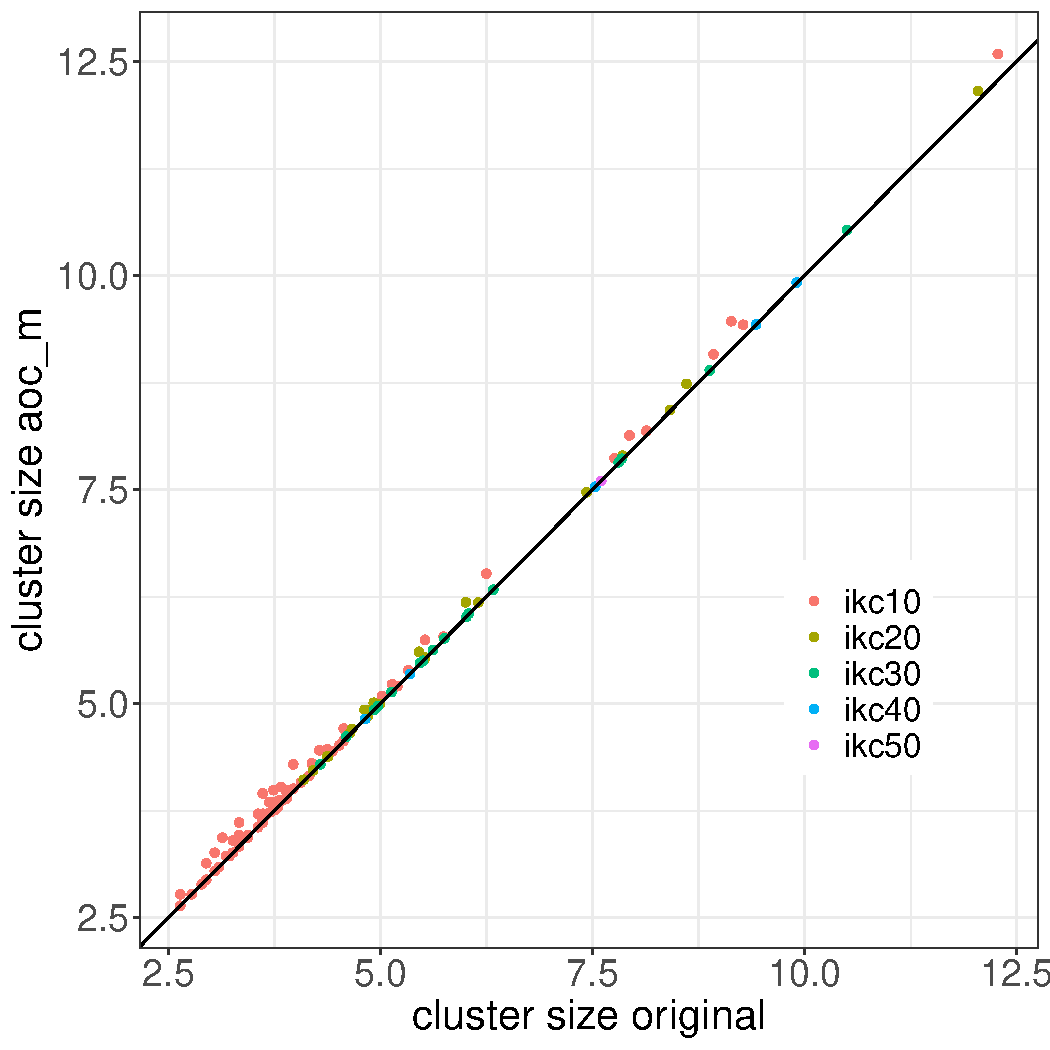
\includegraphics[width=\linewidth]{fig1b.pdf} 
	 %\caption{Generic fig2 a caption} \label{fig:2a}
	 \end{subfigure}
 \hfill
	\begin{subfigure}[t]{0.48\textwidth}
        \centering
        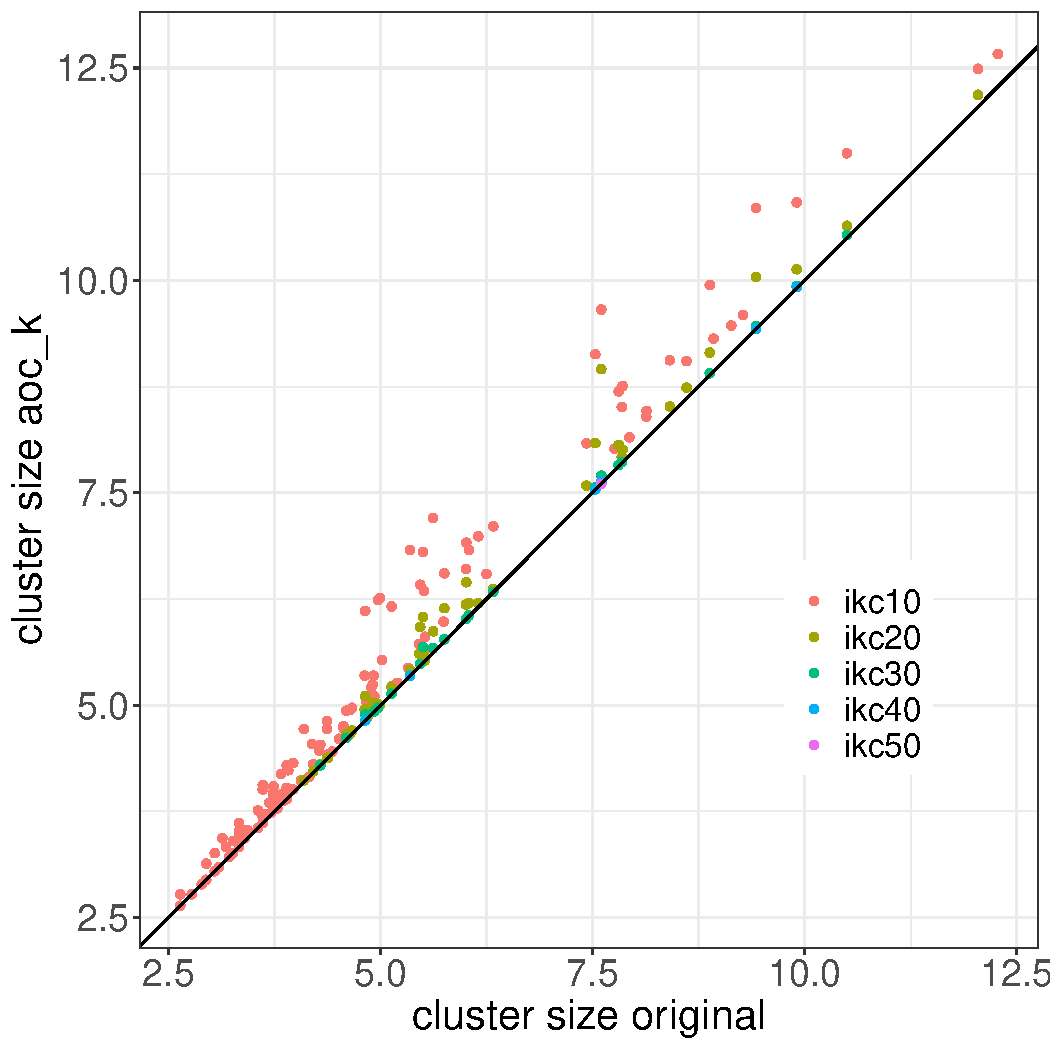
\includegraphics[width=\linewidth]{fig1a.pdf} 
        %\caption{Generic fig2 b caption} \label{fig:2b}
    	\end{subfigure}
\caption{Comparison of cluster sizes between disjoint (IKC)  and overlapping (AOC) clusters (i.e., cluster size increases after enrichment through AOC). Clusters were generated from the CEN network by IKC using values of $k$ ranging from 10 to 50. These clusters were then enriched through the AOC process enforcing either \emph{mcd} (left panel) or \emph{k} (right panel). 
The input to AOC was the  clustering produced by IKC, the value $k$ used to construct the clustering, and the set of nodes to be distributed to additional clusters was all the nodes in the IKC clusters.  Points that lie on the diagonal indicate no change in cluster size after AOC treatment. A natural log scale is used for both axes.}
\label{fig:fig1}
\end{figure}

We then examined the distribution of clusters per candidate node after AOC treatment of clusterings generated by  IKC with $k \in \{10, 20, 30, 40, 50\}$. For AOC\_k treatment of IKC\_k10 cluster, approximately 46\% of the nodes were assigned to a single clusters. The remaining 54\% nodes were assigned to between 2 and 24 clusters in progressively decreasing counts each with roughly 26\% of nodes assigned to 2 clusters and only 1 node being assigned to 24 different clusters (Table~\ref{tab:tab2}). AOC\_m in comparison to AOC\_k, results in fewer multiple cluster assignments because of its more stringent membership criterion (Table~\ref{tab:tab2} and Figure~\ref{fig:fig2}).

\begin{figure}[H]
	\centering
	\begin{subfigure}[t]{0.48\textwidth}
	 \centering
	 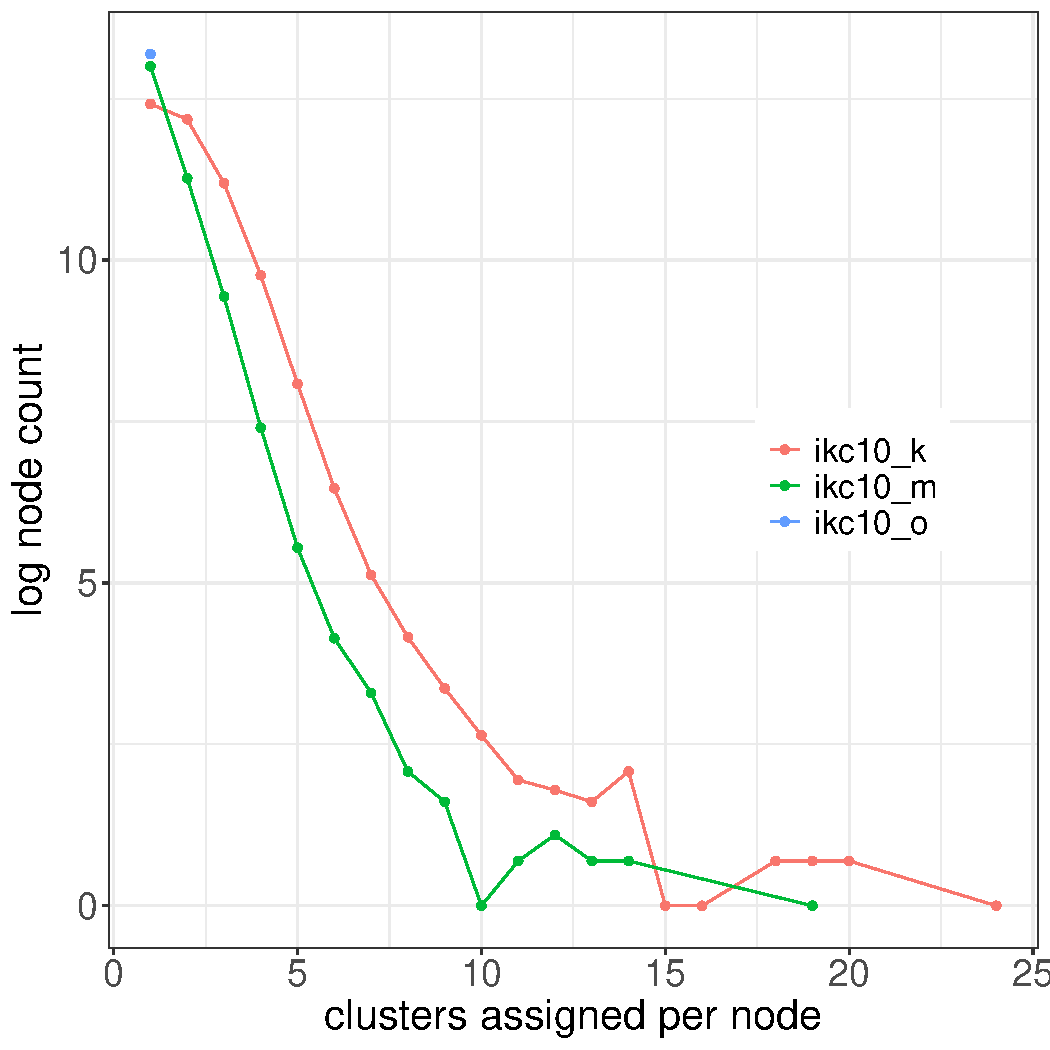
\includegraphics[width=\linewidth]{fig2a.pdf} 
	 %\caption{Generic fig2 a caption} \label{fig:2a}
	 \end{subfigure}
 \hfill
	\begin{subfigure}[t]{0.48\textwidth}
        \centering
        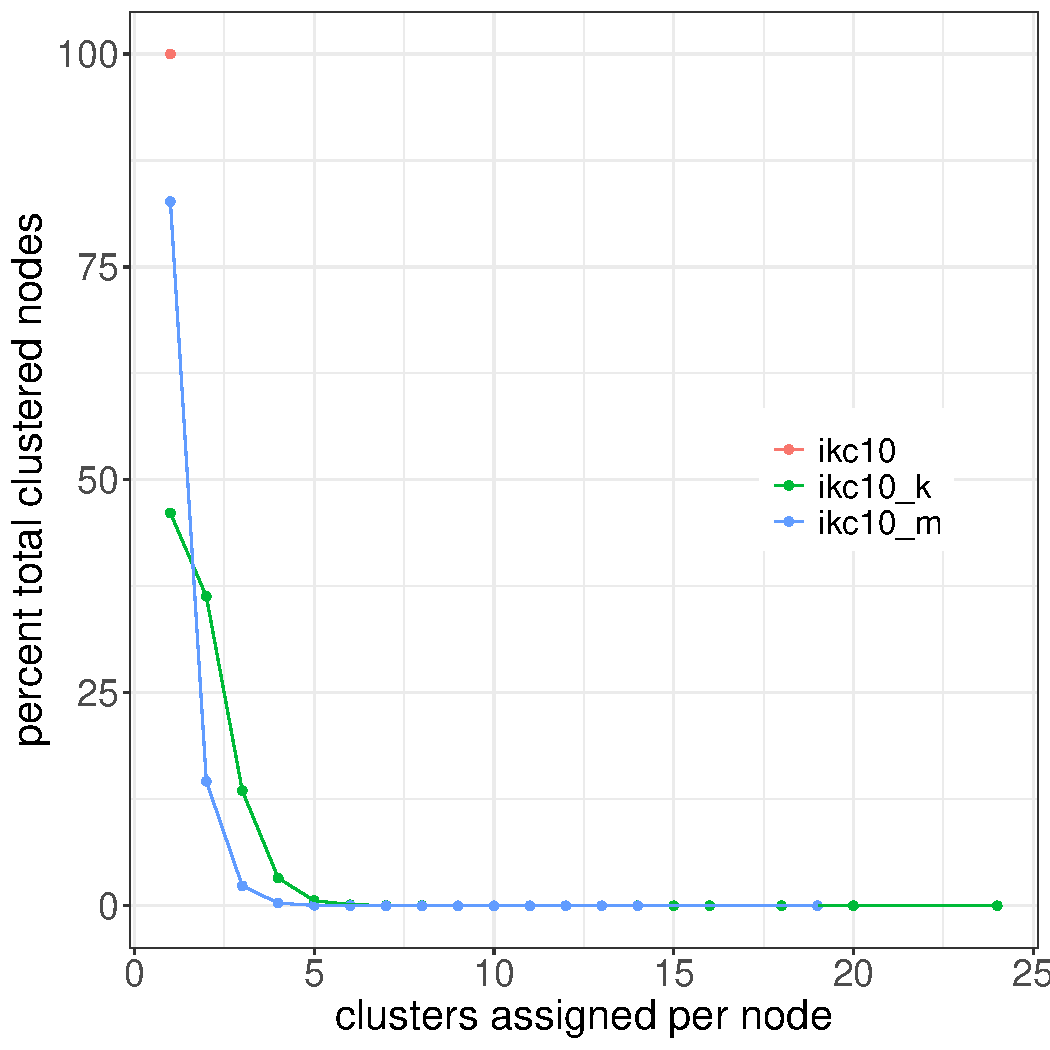
\includegraphics[width=\linewidth]{fig2b.pdf} 
        %\caption{Generic fig2 b caption} \label{fig:2b}
    	\end{subfigure}
\caption{Nodes are assigned to multiple clusters. The figure shows the count of nodes (abscissa) grouped by how many clusters a node was assigned to after AOC treatment enforcing either \emph{k} or \emph{mcd};  these are shown as log counts (left panel) or percentages of the number of nodes (right panel) in non-singleton clusters. 
The single point noted for IKC10\_o indicates that it produced only one non-singleton cluster. I NEED TO CHANGE THE LEGEND from ikc10\_x to aoc\_x}
\label{fig:fig2}
\end{figure}


\subsection{Experiment 3: Which node properties impact multiple assignments?}

\textcolor{blue}{We need something here about total degree correlation with number of clusters, perhaps with number of tier 1 cluster memberships? Something.}


\subsection{Experiment ??: Examining overlap between clusters}
\textcolor{blue}{George, what experiment does this belong in?}
\begin{figure}[H]
	\centering
	\begin{subfigure}[t]{0.48\textwidth}
	 \centering
	 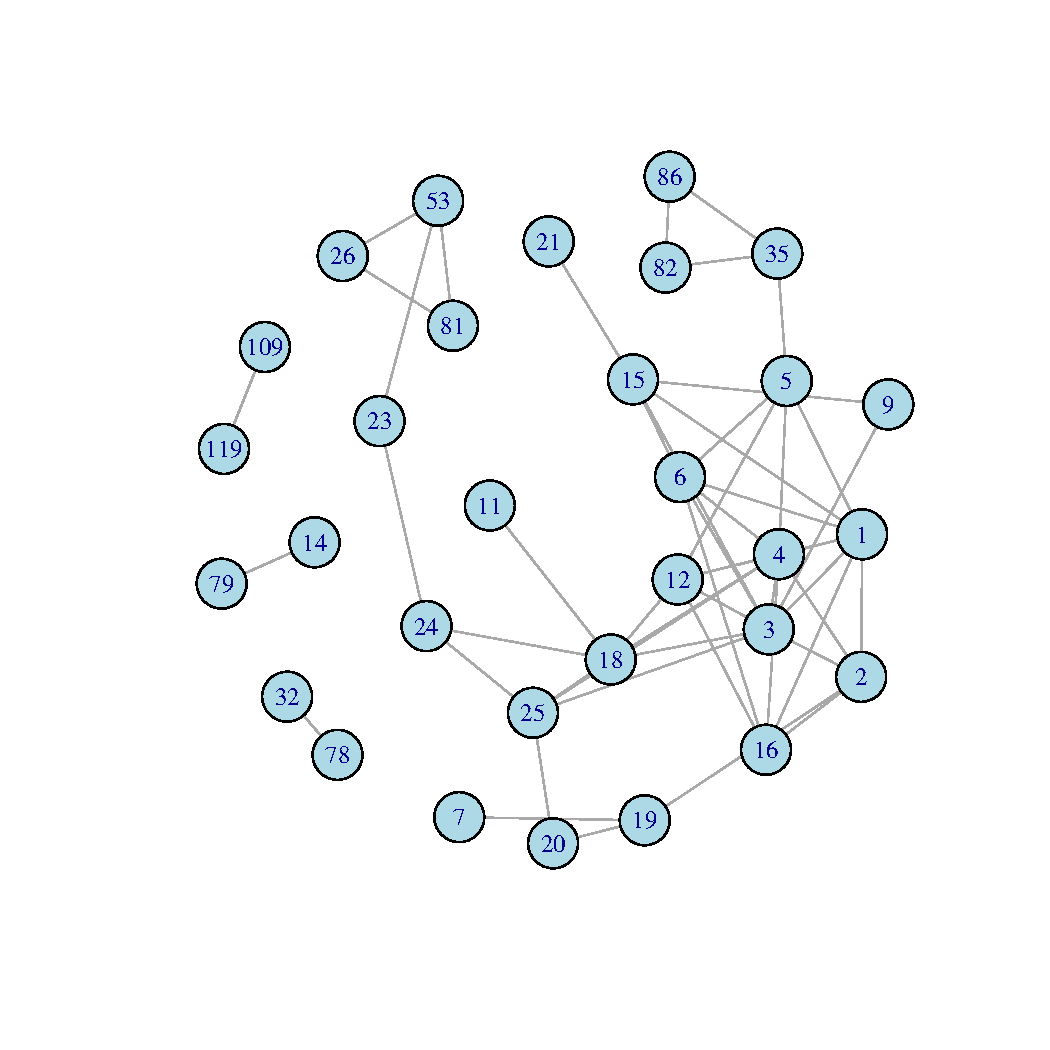
\includegraphics[width=\linewidth]{ikc10_k_pw.pdf} 
	 %\caption{Generic fig2 a caption} \label{fig:2a}
	 \end{subfigure}
 \hfill
	\begin{subfigure}[t]{0.48\textwidth}
        \centering
        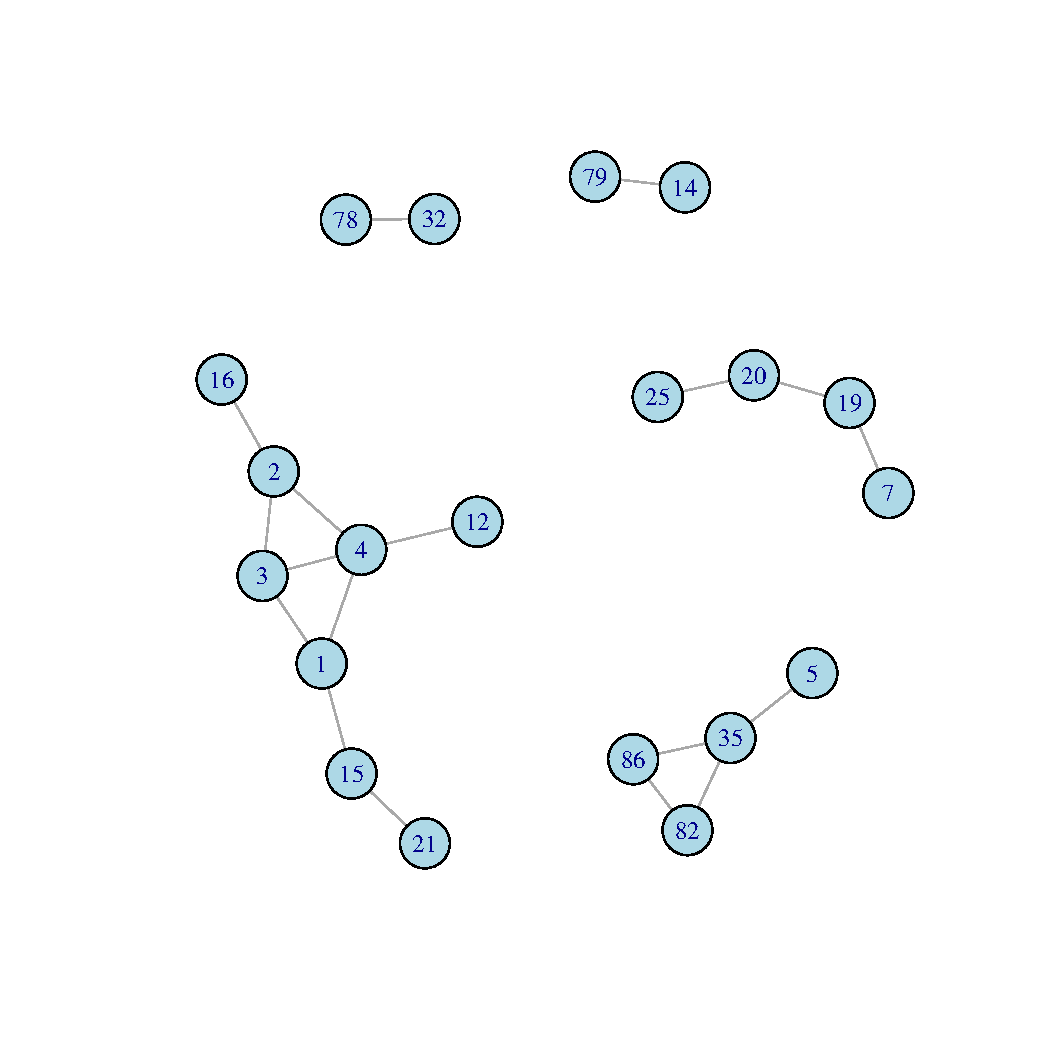
\includegraphics[width=\linewidth]{ikc10_m_pw.pdf} 
        %\caption{Generic fig2 b caption} \label{fig:2b}
    	\end{subfigure}
\caption{Overlapping clusters produced by IKC(10)+AOC.  Clusters were generated from CEN data by IKC using $k=10$. These clusters were then enriched through the AOC process enforcing either \emph{k} (left panel) or \emph{mcd} (right panel). 
The clusters produced  by this two-step process are overlapping. We present information about overlap between these clusters using edges and thickness reflecting how much they overlap; only pairs that have overlap Jaccard Coefficient greater  than the median  non-zero overlap Jaccard Coefficient are connected by edges. 
Cluster numbers in both panels retain cluster numbers from the input IKC clustering.}
\label{fig:fig3}
\end{figure}

\subsection{Experiment 4: Marker node concentrations}

\begin{figure}[H]
	\centering
	 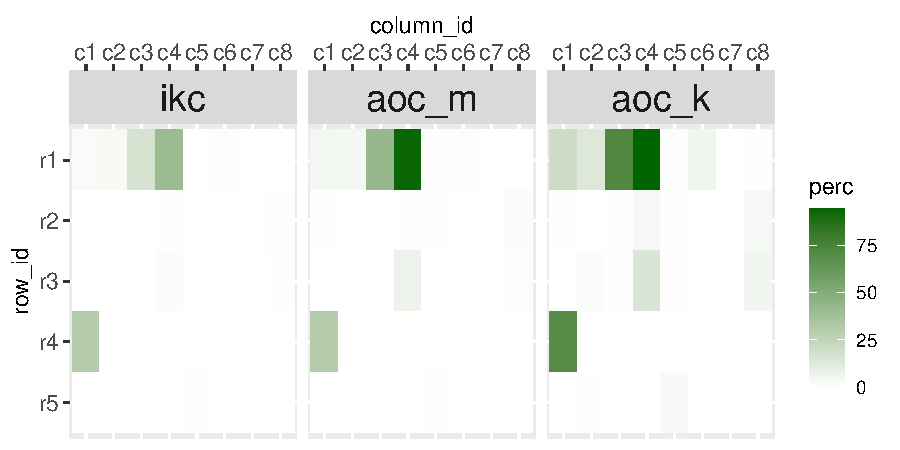
\includegraphics[width=0.7\linewidth]{marker_comps_wide.pdf} 
\caption{AOC increases marker node concentration. We show marker node counts in 40 clusters (5 rows with 8 clusters per row) before and after AOC.  Notably, the proportion of 1021 marker nodes in the network increases from 40.7\% in cluster 4 (r1,c4) of IKC clustering to 93.1\% after AOC\_m to 94.6\% after AOC\_k. The proportion of markers in cluster 25 (r4,c1) is the same for IKC and AOC\_m but increases to  69.5\% under the more permissive conditions of AOC\_m. (Data are shown for the 40 clusters with non-zero marker node counts in IKC. Data for all 128 clusters are available in Supplementary Material.)}
\label{fig:fig4}
\end{figure}

\clearpage
\begin{table}[H]
\centering
\begin{tabular}{rlcc}
  \hline
 & AOC\_m & no\_change & increase \\ 
  \hline
1 & ikc10 &  33 &  95 \\ 
2 & ikc20 &  10 &  34 \\ 
3 & ikc30 &   8 &  14 \\ 
4 & ikc40 &   3 &   3 \\ 
5 & ikc50 &   1 &   0 \\ 
   \hline
\end{tabular}
\quad
\begin{tabular}{rlcc}
  \hline
 & AOC\_k& no\_change & increase \\ 
  \hline
1 & ikc10 &  17 & 111 \\ 
2 & ikc20 &   2 &  42 \\ 
3 & ikc30 &   4 &  18 \\ 
4 & ikc40 &   2 &   4 \\ 
5 & ikc50 &   1 &   0 \\ 
   \hline
\end{tabular}
\caption{\textcolor{blue}{George, what is this table about? I don't know..}}
\label{tab:tab1}
\end{table}

\clearpage
\begin{sidewaystable}[h!]
\centering
\resizebox{\textwidth}{!}{
\begin{tabular}{clllllllllll}
  \hline
 no\_clusters & ikc10\_k & ikc10\_m & ikc20\_k & ikc20\_m & ikc30\_k & ikc30\_m & ikc40\_k & ikc40\_m & ikc50\_k & ikc50\_m \\ 
  \hline
1 & 246787 & 442485 & 221728 & 254435 & 85515 & 86806 & 36367 & 36463 & 2004 & 2004 \\ 
2 & 194427 & 78150 & 49195 & 20280 & 2731 & 1487 & 363 & 269 &  &  \\ 
3 & 72367 & 12518 & 4511 & 1057 &  82 &  43 &   4 &   2 &  &  \\ 
4 & 17401 & 1642 & 377 &  98 &  15 &   8 &  &  &  &  \\ 
5 & 3232 & 256 &  61 &  21 &   2 &   1 &  &  &  &  \\ 
6 & 641 &  63 &  19 &   5 &  &  &  &  &  &  \\ 
7 & 168 &  27 &   4 &  &  &  &  &  &  &  \\ 
8 &  64 &   8 &   1 &   1 &  &  &  &  &  &  \\ 
9 &  29 &   5 &   1 &  &  &  &  &  &  &  \\ 
10 &  14 &   1 &   1 &   1 &  &  &  &  &  &  \\ 
11 &   7 &   2 &  &  &  &  &  &  &  &  \\ 
12 &   6 &   3 &  &  &  &  &  &  &  &  \\ 
13 &   5 &   2 &  &  &  &  &  &  &  &  \\ 
14 &   8 &   2 &  &  &  &  &  &  &  &  \\ 
15 &   1 &  &  &  &  &  &  &  &  &  \\ 
16 &   1 &  &  &  &  &  &  &  &  &  \\ 
18 &   2 &  &  &  &  &  &  &  &  &  \\ 
19 &   2 &   1 &  &  &  &  &  &  &  &  \\ 
20 &   2 &  &  &  &  &  &  &  &  &  \\ 
24 &   1 &  &  &  &  &  &  &  &  &  \\ 
   \hline
\end{tabular}}
\caption{Cluster Size Increases After AOC Treatment. The count of clusters that either increase in size (increase) or remain the same size (no\_change) is shown
for either AOC\_m (left) or AOC\_k (right) treatment for five different values of $k$ and where the nodes allowed to be in multiple clusters are those that appear in one non-singleton cluster in IKC(k). 
 For k=50, IKC returns a single cluster; by definition, the cluster does not change after AOC treatment.}
\label{tab:tab2}
\end{sidewaystable}

\clearpage







\subsection{Equilibration Across Cores}

\subsection{Nodes of High Degree}

\subsection{Enforcing MCD}

\subsection{Data}

\section{Conclusions}
\section{Acknowledgments etc.}

\bibliographystyle{apalike}
\bibliography{akhil.bib}

\end{document}
%%%%%%%%%%%%%%%%
%%%%%%%%%%%%%%%%
%%%%%%%%%%%%%%%%
%%%%%%%%%%%%%%%%


\textbf{ Introduce the Problem of Clustering for Bibliometrics}
\begin{itemize}
	\item Trying to identify specific communities from a larger network of publications within an overarching field
	\item Attempts to solve this problem within the lensof citation networks which means through the connections of publications based on how they cite/reference other publications within their field
	\item Focal publications can be part of many separate communities like BLAST can and should be part of many smaller communities but disjoint clustering methods leave out this possibility 
	\item Price and Beaver, Wedell et al mention the impact of a core and periphery structure, for which can we analyze the impact of overlapping clusters on the core structure
 \end{itemize}
 
 
\subsection{Center-periphery communities}

Discuss Price \& Beaver \cite{price_1966} and anything else that is related to center-periphery structure in communities.

\subsection{kmp-clustering }

The method from Wedell et al. \cite{Wedell2022} seeks to  cluster a graph into disjoint clusters, each of which 
exhibits center-periphery structure, as specified by numeric parameters $k$ and $p$ that are provided by the user.
Specifically, a cluster is said to be $k$-valid if... and $p$-valid if... and $m$-valid if...


The kmp-clustering pipeline developed in \cite{Wedell2022}  performs this clustering, based on the user provided values for $k$ and $p$, and has the following four steps: 
\begin{itemize}
	\item Step 1: IKC(N,k): producing a set of disjoint clusters, each of which is k-valid.
	\item Step 2 (optional). Divide into smaller clusters, Recursive Graclus
	\item Step 3 (optional): Augment for Periphery
	\item Step 4 (not optional): parse again, making sure to update for kmp-validity
\end{itemize}


\subsection{Overlapping clustering methods}

Here we summarize the existing methods for overlapping clusters.

\paragraph{Lambiotte and Evans}

\paragraph{Others?}

\section{Study Design}
\subsection{Overview}
We have developed a variant of the kmp-clustering method from Wedell et al. \cite{Wedell2022} that is designed to produce overlapping
clusters.
We refer to this as Overlapping kmp-clustering, or OKMP for short\footnote{This is an awful name and we should change it!}
Like kmp-clustering, the user provides values for the parameters $k$ and $p$ and the method is guaranteed to output
clusters that are $kmp$-valid.
However, unlike kmp-clustering, we allow nodes to be members of more than one cluster; as a result, the output is a clustering where
the clusters can be overlapping.

We study OKMP  in comparison to KMP-clustering (which by design produces disjoint clusters). 
We also compare OKMP to  other methods that are designed to produce overlapping clusters.
We evaluate methods on two citation networks that we construct, both developed for the Exosome biology research community.
We report empirical statistics, such as node coverage and edge coverage, and also explore cluster size.
We specifically explore the number of clusters that each publication belongs to, and evaluate the correlation between
citation count and cluster membership.
We examine pairs of overlapping clusters to understand how allowing for multiple memberships provides more insight into community
structure.



\subsection{Clustering Methods}
The main focus of this paper is the new clustering method that we have developed, Overlapping kmp-clustering, which we refer to as OKMP for short.
We also compare OKMP to other methods, which we describe below.

\subsubsection{Overlapping kmp-clustering}

\textbf{Talk about New Stage 5}

What we propose to do is add a Step 5 that will achieve overlapping clusters. More generally, the Step 5 will be able to be used with any input clustering (even if not disjoint) of a network N. And if given values for k and p, will maintain kmp-validity, if desired. Furthermore, we have a variant of this Step 5 that will maintain MCD (minimum core degree).

\textbf{Proposed greedy algorithm}

Suppose we have as input a network $N$, values for $k$ and $p$, and a clustering $\mathcal{C}$, and we want to now allow for nodes to be members in more than one cluster.  Thus we want to enhance $\mathcal{C}$ to create a new clustering, but using $\mathcal{C}$ as a starting point.
Here is a general technique:

\begin{itemize}
	\item Sort the nodes of $N$ according to some criterion (the studies mention in this paper will sort by total degree of the publication in the network)
	\item Process the nodes in order of this criterion, from best to worst, until a stopping condition applies (could be the size of the resulting clustering, or amount of time that has passed)
	\begin{itemize}
		\item Given node $v$, add $v$ to any cluster in $C \in \mathcal{C}$ where $v$ has at least $k$ neighbors (alternatively, 
		$v$ has at least $MCD(C)$ neighbors) among the core elements of $C$.
	\end{itemize}
\end{itemize}

In the current version of this algorithm, when we add a node to a cluster, we do not add the node as a core member and thus we only need to iterate over the cluster once to add all nodes



\subsubsection{Line Graph Method}

From Evans and Lambiotte, a method of overlapping clustering was proposed that involves computing the line graph equivalent of a given network and running a disjoint clustering algorithm like Leiden on the resulting line graph. 
\begin{itemize}
	\item Step 1: LG(N): produce a network where edges represent nodes, nodes represents edges
	\item Step 2 Cluster(LG(N)). Run disjoint clustering algorithm on the line graph
\end{itemize}

Talk about scalability issues of Method


\subsection{Experiments}

 
Recall that OKMP depends on the values for $k$ and $p$, but in this initial experiment we do not 
consider periphery membership, and so $p$ is irrelevant.
It also depends on which publications are allowed to be
put in more than one cluster; for our algorithm, this is mainly based on modifying $N$ where 
we order the nodes based on total degree and then only allow the top $N$ nodes to be in multiple clusters.
However, we also have a variant where we process a user-provided set of nodes, which could be all the nodes in a specific cluster, or  all the marker nodes, etc. 
Finally, OKMP depends on the rule for allowing a node to join a new cluster: do we only enforce k-validity, or do
we enforce MCD values (where MCD stands for Minimum Cluster Degree)? Here we note the MCD value of a cluster is
always (by definition) at least $k$, so that enforcing MCD is a stronger requirement, and may result in a node being added to
fewer clusters.


\textcolor{blue}{Akhil - does Stage 1 check for positive modularity? When we do Experiment 0, are we checking for positive modularity? Ditto for Experiment 1.}

\begin{itemize}
\item 
Experiment 0: Characterize step 1 of kmp-processing (i.e., we only do IKC(k)) for $k$ ranging from $10$ to $50$. These will be used
in subsequent experiments.
\item Experiment 1:  Look at OKM-clustering for different values of $k$ and for a specific set of nodes for processing. That set of nodes
will be the top $N$ nodes based on total degree or something else. For this, we only look at enforcing km-validity (not MCD).  Probably we use the top1\% of the nodes in terms of total degree for this set. 
\item Experiment 2:  Based on experiment 1, we will fix the value for $k$ (to at most two values), and now vary the set of  nodes for processing.
Here we make some discoveries about this kind of overlapping clustering.
\item Experiment 3: vary MCD vs k-m-validity to decide differences in sights.
\item Experiment 4: Take best settings so far, but break up the largest clusters (i.e., add back in the Stage 2 using Recursive Graclus).
\item Experiment 5: Allow for periphery.
\end{itemize}

In each experiment, we report:
\begin{itemize}
\item Characteristics of the set of nodes that are only in singleton clusters
\item Node coverage
\item Edge coverage
\item Cluster size distributions
\item Overlap between clusters
\end{itemize}

We show various empirical statistics of the clustering,  including the number of non-singleton clusters, the number of singleton clusters, the minimum, median and maximum cluster sizes,  node and edge coverage of the network, and node and edge coverage of the marker node subnetwork.


\section{Results \& Discussion}

\subsection{Explaining the Quantitative Metrics}
We can begin by giving a description of all metrics evaluated in the following two tables. The Number of Non-Singleton Clusters represents the number of clusters generated with at least 2 nodes in the cluster. The number of Singleton Clusters represents the number of nodes not present in any of the non-singleton clusters. The minimum cluster size represents the size of smallest non-singleton cluster generated. Similarly, the median and maximum cluster size represent the size of the median and largest non-singleton cluster generated respectively. Node Coverage is calculated by finding the percentage of nodes found in a non-singleton cluster compared to the total number of nodes in the network. Similarly, edge coverage is calculated by finding the total number of edges found in non-singleton clusters (both endpoint nodes are found in the cluster) compared to the total number of edges found in the network. We can use the same process to define marker node coverage and marker edge coverage. Marker node coverage represents the percentage of marker nodes found in non-singleton clusters compared to the total amount of marker nodes (n=95). Marker edge coverage represents the percentage of all edges that can be found in non-singleton clusters where both endpoint nodes of the edge are in the cluster (with at least one endpoint being a marker node) compared to the total edges of marker nodes. 
\newline

Results for Experiment 0 are shown in Table \ref{table:expt0}. This experiment runs the original disjoint IKC clustering method for k-values in the range of $\{10, 20, 30, 40, 50\}$. We show various empirical statistics of the clustering,  including the number of non-singleton clusters, the number of singleton clusters, the minimum, median and maximum cluster sizes,  node and edge coverage of the network, and node and edge coverage of the marker node subnetwork.

\begin{table}[h!]
\centering
\begin{small}
	\begin{tabular}{ |p{0.95cm}||p{1.25cm}|p{1.25cm}||p{1.20cm}|p{1.20cm}|p{1.20cm}||p{1.25cm}|p{1.25cm}|| p{1.25cm}|p{1.25cm}||p{0.95cm}| }
		\hline
		\multicolumn{11}{|r|}{Experiment 0} \\
		\hline
		Method & Number of Non-Singleton Clusters & Number of Singleton Clusters & Minimum Cluster Size &  Median Cluster Size & Maximum Cluster Size & Node Coverage (\%)& Edge Coverage  (\%)& Marker Node Coverage  (\%)& Marker Edge Coverage  (\%) & Elapsed Time (min:s) \\
		\hline
		IKC (k=10)   &  \textbf{128}    & 13454271 &   14 & 79.0 & \textbf{214877} & \textbf{3.83\%} & \textbf{11.8\% }& \textbf{89.5\% }& \textbf{8.33\% }& 26:46\\ \hline
		IKC (k=20)   &  44    & 13713538 &   60 & 246.5 & 170413 & 1.97\% & 8.24\% & 48.4\% & 6.62\% & 26:11\\ \hline
		IKC (k=30)   &  22    & 13901091 &   73 & 361.5 & 36305 & 0.63\% & 3.33\% & 42.1\% & 6.35\% & 25:22\\ \hline
		IKC (k=40)   &  6    & 13952702 &   124 & 1936.5 & 20076 & 0.26\% & 1.61\% & 41.1\% & 6.29\% & 26:01\\ \hline
		IKC (k=50)   &  1    & \textbf{13987432} &   \textbf{2004} & \textbf{2004.0} & 2004 & 0.01\% & 0.11\% & 0.00\% & 0.00\% & 24:46\\ \hline
		\hline
	\end{tabular}
	\end{small}
	\caption{Results for Experiment 0. In this experiment we run IKC on different values for $k$ between $10$ and $50$, and we report different
	empirical statistics. Note that this experiment produces disjoint clustering, and is equivalent to running Stage 1 of the $kmp$-clustering method of Wedell et al. (2022).}
		\label{table:expt0}
\end{table}

\begin{table}[h!]
\centering
\begin{small}
	\begin{tabular}{ |p{0.95cm}||p{1.25cm}|p{1.25cm}||p{1.20cm}|p{1.20cm}|p{1.20cm}||p{1.25cm}|p{1.25cm}|| p{1.25cm}|p{1.25cm}||p{0.95cm}| }
		\hline
		\multicolumn{11}{|c|}{Experiment 1} \\
		\hline
		Method & Number of Non-Singleton Clusters & Number of Singleton Clusters & Minimum Cluster Size &  Median Cluster Size & Maximum Cluster Size & Node Coverage (\%)& Edge Coverage  (\%)& Marker Node Coverage  (\%)& Marker Edge Coverage  (\%) & Elapsed Time (s)\\
		\hline
		IKC (k=10) w/ Step 5   &  \textbf{128}    & 13446836 &   14 & 85.0 & \textbf{275688} & \textbf{3.88\%} & \textbf{19.1\% }& \textbf{89.5\% }& \textbf{25.3\%} & 39:43\\ \hline
		IKC (k=20)  w/ Step 5 &  44    & 13702335 &   61 & 278.0 & 194798 & 2.05\% & 11.3\% & 53.7\% & 14.0\% & 29:25\\ \hline
		IKC (k=30)  w/ Step 5 &  22    & 13894563 &   73 & 388.5 & 38260 & 0.68\% & 3.80\% & 46.3\% & 7.66\% & 28:26\\ \hline
		IKC (k=40)  w/ Step 5 &  6    & 13951394 &   130 & 2299.0 & 20488 & 0.27\% & 1.70\% & 44.2\% & 6.82\% & 26:59\\ \hline
		IKC (k=50) w/ Step 5  &  1    & \textbf{13987362} &   \textbf{2074} & \textbf{2074.0} & 2074 & 0.01\% & 0.11\% & 0.00\% & 0.00\% & 25:16\\ \hline
		\hline
	\end{tabular}
	\end{small}
	\caption{Results for Experiment 1. This is the result of running IKC for different values of $k$ and then allowing some nodes to be members in multiple clusters. The set of nodes that are allowed to belong to multiple clusters is the top 1\% of nodes, by total degree. These are placed independently of each other, and so order does not matter.  Membership in a new cluster requires that the added node be adjacent to at least $k$ other nodes in the IKC cluster (thus, newly added nodes do not vote on membership for other new nodes)}
	\label{table:expt1}
\end{table}


\begin{table}[h!]
	\centering
	\begin{small}
		\begin{tabular}{ |p{0.95cm}||p{1.25cm}|p{1.25cm}||p{1.20cm}|p{1.20cm}|p{1.20cm}||p{1.25cm}|p{1.25cm}|| p{1.25cm}|p{1.25cm}| }
			\hline
			\multicolumn{10}{|c|}{Experiment 2 Indegree} \\
			\hline
			Method & Number of Non-Singleton Clusters & Number of Singleton Clusters & Minimum Cluster Size &  Median Cluster Size & Maximum Cluster Size & Node Coverage (\%)& Edge Coverage  (\%)& Marker Node Coverage  (\%)& Marker Edge Coverage  (\%)\\
			\hline
			IKC (k=20)  w/ Step 5 In-degree $1\%$ &  44    & \cellcolor{blue!20} 13702262 &   61 & \cellcolor{red!20} 280.5 & \cellcolor{blue!20}192690 & 2.05\% & \cellcolor{blue!20}11.0\% & \cellcolor{blue!20}52.6\% & \cellcolor{blue!20}13.6\% \\ \hline

			IKC (k=40)  w/ Step 5 In-degree $1\%$ &  6    & \cellcolor{red!20}13951603 &   \cellcolor{red!20}131 & \cellcolor{red!20}2235.5 & \cellcolor{blue!20}20462 & 0.27\% & \cellcolor{blue!20}1.69\% & \cellcolor{blue!20}42.1\% & \cellcolor{blue!20}6.52\% \\ \hline
			
			IKC (k=20)  w/ Step 5 In-degree $5\%$&  44    & \cellcolor{blue!20}13621558 &   61 & \cellcolor{red!20}450.0 & \cellcolor{red!20}229928 & \cellcolor{red!20}2.63\% & \cellcolor{red!20}14.5\% & \cellcolor{red!20}72.6\% & \cellcolor{red!20}17.7\% \\ \hline
			
			IKC (k=40)  w/ Step 5 In-degree $5\%$ &  6    & \cellcolor{blue!20}13949455 &   \cellcolor{red!20}139 & \cellcolor{red!20}2645.0 & \cellcolor{red!20}21002 & \cellcolor{red!20}0.29\% & \cellcolor{red!20}1.80\% & \cellcolor{red!20}47.4\% & \cellcolor{red!20}7.29\% \\ \hline

			 \hline
			\hline
					\end{tabular}
		\end{small}
	\caption{Results for Experiment 2. We now decide to fix k=20, 40 and vary the input candidate set. We take a look at the following variations:  changing the candidate criterion to in-degree instead of total degree and looking at the top $1\%$ of nodes and top $5\%$ of nodes respectively. }
	\label{table:expt2indegree}
\end{table}

\begin{table}[h!]
	\centering
	\begin{small}
		\begin{tabular}{ |p{0.95cm}||p{1.25cm}|p{1.25cm}||p{1.20cm}|p{1.20cm}|p{1.20cm}||p{1.25cm}|p{1.25cm}|| p{1.25cm}|p{1.25cm}| }
			\hline
			\multicolumn{10}{|c|}{Experiment 2 Total Degree} \\
			\hline
			Method & Number of Non-Singleton Clusters & Number of Singleton Clusters & Minimum Cluster Size &  Median Cluster Size & Maximum Cluster Size & Node Coverage (\%)& Edge Coverage  (\%)& Marker Node Coverage  (\%)& Marker Edge Coverage  (\%)\\
			\hline
			IKC (k=20)  w/ Step 5 Total Degree $5\%$&  44    & \cellcolor{blue!20}13603978 &   \cellcolor{red!20}62 & \cellcolor{red!20}480.5 & \cellcolor{red!20}232822 &\cellcolor{red!20}2.76\% & \cellcolor{red!20}15.7\% & \cellcolor{red!20}77.9\% & \cellcolor{red!20}21.7\%  \\ \hline
			
			IKC (k=40)  w/ Step 5 Total Degree $5\%$ &  6    & \cellcolor{blue!20}13948073 &   \cellcolor{red!20}144 & \cellcolor{red!20}2909.0 & \cellcolor{red!20}21345 & \cellcolor{red!20}0.30\% & \cellcolor{red!20}1.87\% & \cellcolor{red!20}48.4\% & \cellcolor{red!20}8.10\% \\
			\hline
			\hline
		\end{tabular}
	\end{small}
	\caption{Results for Experiment 2. We now decide to fix k=20, 40 and vary the input candidate set. We take a look at the following variations:  changing the candidate criterion to the  top $5\%$ of nodes by total degree.}
	\label{table:expt2totaldegree}
\end{table}

\begin{table}[h!]
	\centering
	\begin{small}
		\begin{tabular}{ |p{0.95cm}||p{1.25cm}|p{1.25cm}||p{1.20cm}|p{1.20cm}|p{1.20cm}||p{1.25cm}|p{1.25cm}|| p{1.25cm}|p{1.25cm}| }
			\hline
			\multicolumn{10}{|c|}{Experiment 2 Random} \\
			\hline
			Method & Number of Non-Singleton Clusters & Number of Singleton Clusters & Minimum Cluster Size &  Median Cluster Size & Maximum Cluster Size & Node Coverage (\%)& Edge Coverage  (\%)& Marker Node Coverage  (\%)& Marker Edge Coverage  (\%)\\
			\hline
			IKC (k=20)  w/ Step 5 Random &  44    & \cellcolor{red!20}13711657 &   \cellcolor{blue!20}60 & \cellcolor{blue!20}250.0 & \cellcolor{blue!20}171448 & \cellcolor{blue!20}2.00\% & \cellcolor{blue!20}8.32\% & \cellcolor{blue!20}49.5\% & \cellcolor{blue!20}6.72\% \\ \hline
			
			IKC (k=40)  w/ Step 5 Random  &  6    & \cellcolor{red!20}13952652 &   \cellcolor{blue!20}124 & \cellcolor{blue!20}1946.0 & \cellcolor{blue!20}20090 & \cellcolor{blue!20}0.26\% & \cellcolor{blue!20}1.61\% & \cellcolor{blue!20}41.1\% & \cellcolor{blue!20}6.31\% \\ \hline
			\hline
		\end{tabular}
	\end{small}
	\caption{Results for Experiment 2. We now decide to fix k=20, 40 and vary the input candidate set. We take a look at the following variations:  changing the candidate criterion to a random $1\%$ of nodes from the network. }
	\label{table:expt2random}
\end{table}

\begin{table}[h!]
	\centering
	\begin{small}
		\begin{tabular}{ |p{0.95cm}||p{1.25cm}|p{1.25cm}||p{1.20cm}|p{1.20cm}|p{1.20cm}||p{1.25cm}|p{1.25cm}|| p{1.25cm}|p{1.25cm}| }
			\hline
			\multicolumn{10}{|c|}{Experiment 2 95th Percentile} \\
			\hline
			Method & Number of Non-Singleton Clusters & Number of Singleton Clusters & Minimum Cluster Size &  Median Cluster Size & Maximum Cluster Size & Node Coverage (\%)& Edge Coverage  (\%)& Marker Node Coverage  (\%)& Marker Edge Coverage  (\%)\\
			\hline
			IKC (k=20)  w/ Step 5 Total Degree 95 Percentile &  44    & \cellcolor{blue!20}13684128 &   61 & \cellcolor{blue!20}268.5 & \cellcolor{blue!20}180166 & \cellcolor{red!20}2.18\% & \cellcolor{blue!20}9.04\% & \cellcolor{blue!20}49.5\% & \cellcolor{blue!20}6.92\% \\ \hline
			
			IKC (k=40)  w/ Step 5 Total Degree 95 Percentile  &  6    & \cellcolor{red!20}13952552 &   \cellcolor{blue!20}124 & \cellcolor{blue!20}1940.0 & \cellcolor{blue!20}20170 & \cellcolor{blue!20}0.26\% & \cellcolor{blue!20}1.62\% & \cellcolor{blue!20}41.1\% & \cellcolor{blue!20}6.29\% \\ \hline
			\hline
			IKC (k=20)  w/ Step 5 Indegree 95 Percentile &  44    & \cellcolor{blue!20}13700075 &   \cellcolor{blue!20}60 & \cellcolor{blue!20}253.0 & \cellcolor{blue!20}176775 & \cellcolor{red!20}2.07\% & \cellcolor{blue!20}8.64\% & \cellcolor{blue!20}49.5\% & \cellcolor{blue!20}7.02\% \\ \hline
			
			IKC (k=40)  w/ Step 5 Indegree 95 Percentile  &  6    &\cellcolor{red!20}13952523 &   \cellcolor{blue!20}125 & \cellcolor{blue!20}1968.0 & \cellcolor{blue!20}20128 & \cellcolor{blue!20}0.26\% & \cellcolor{blue!20}1.62\% &\cellcolor{blue!20}41.1\% & \cellcolor{blue!20}6.34\% \\ \hline
			\hline
		\end{tabular}
	\end{small}
	\caption{Results for Experiment 2. We now decide to fix k=20, 40 and vary the input candidate set. We take a look at the following variations:  changing the candidate criterion to the 95th percentile (94.5-95.5) of nodes by either in-degree or total degree. }
	\label{table:expt2}
\end{table}
			 
\begin{table}[h!]
	\centering
	\begin{small}
		\begin{tabular}{ |p{0.95cm}||p{1.25cm}|p{1.25cm}||p{1.20cm}|p{1.20cm}|p{1.20cm}||p{1.25cm}|p{1.25cm}|| p{1.25cm}|p{1.25cm}| }
			\hline
			\multicolumn{10}{|c|}{Experiment 2 Seed} \\
			\hline
			Method & Number of Non-Singleton Clusters & Number of Singleton Clusters & Minimum Cluster Size &  Median Cluster Size & Maximum Cluster Size & Node Coverage (\%)& Edge Coverage  (\%)& Marker Node Coverage  (\%)& Marker Edge Coverage  (\%)\\
			\hline
			IKC (k=20)  w/ Step 5 Seed &  44    & \cellcolor{blue!20}13526555 &  \cellcolor{red!20} 62 & \cellcolor{red!20}495.0 &\cellcolor{red!20} 270561 & \cellcolor{red!20}3.31\% & \cellcolor{red!20}18.1\% & \cellcolor{red!20}77.9\% & \cellcolor{red!20}22.6\% \\ \hline
			
			IKC (k=40)  w/ Step 5 Seed  &  6    & \cellcolor{blue!20}13948032 &   \cellcolor{red!20}144 & \cellcolor{red!20}2910.5 & \cellcolor{red!20}21371 & \cellcolor{red!20}0.30\% &\cellcolor{red!20}1.87\% & \cellcolor{red!20}48.4\% & \cellcolor{red!20}8.10\% \\  \hline
			\hline
		\end{tabular}
	\end{small}
	\caption{Results for Experiment 2 Seed. We now decide to fix k = 20, 40 and vary the input candidate set. We take a look at the following variations:  changing the candidate criterion to the seed set and the marker nodes.}
	\label{table:expt2seed}
\end{table}

	
Experiment 2:
\begin{itemize}
	\item X is a random set of nodes found in clusters \textbf{done}
	\item X is set of publications with top 5$\%$ in terms of degree \textbf{done}
	\item X is the same number of publications at the 95th percentile (94.5-95.5%)
	\item X is the set of publications with top 1$\%$in terms of in-degree \textbf{done}
	\item X is the set of publications with top 5$\%$ in terms of in-degree  \textbf{done}
	\item X is the set of publications between 94.5-95.5$\%$ in terms of in-degree
	\item X is some set of marker nodes. (ALL marker nodes)
		All 1200 from Wedell et al. 2022
		The more recent set of 94 marker nodes
		The set of S nodes
\end{itemize}


\subsection{Observations}

When looking at Experiment 0, which looks at disjoint IKC km-valid clusterings, we notice the trend that as we increase k-value, we restrict our clusters lesser nodes from the network, albeit potentially more informative and connected ones. The number of non-singleton nodes decreases as k increases, while the median and minimum cluster size increase and the maximum cluster size decreases. As the selectivity of the clustering algorithm increases, we notice that the distribution of cluster sizes tends to the median. Node coverage and edge coverage also decrease as the selectivity of the clustering algorithm increases as expected in the inverse relationship between selectivity and coverage. Interestingly, we notice that the marker node coverage is greater than node coverage (which represents all nodes in the graph), while marker edge coverage is actually less that the average node for k=10, k=20 byt bit for large values of k up until k=50. We can attribute this to the fact that increasing selectivity values papers with higher total degrees which in turn tend to be papers with greater significance in their field. Thus marker node abnd edge coverage being proportionally higher for more selective values of k supports this idea. \newline\newline

We can then look at Experiment 1, which looks at the OKMP valid clustering based on the same original disjoint IKC km-valid clusterings from Experiment 0. Given that our algorithm only adds candidate nodes to existing clusters from the input disjoint clusterings, the number of non-singleton clusters stays the same. However, we notice the general trends of increases in minimum, median and maximum cluster sizes, and decreases in singleton clusters. These trends continue to show in node and edge coverage which both increase for all k-values. Given that this stage takes the set of the top $1\%$ of nodes by total degree to be considered when adding to existing clusters, we can notice that the maximum increase of node coverage is bounded at $1\%$. We also notice that unlike Experiment 0, the marker edge coverage exceeds the edge coverage for all k-values (except k=50), which gives evidence that points to OKMP valuing these marker nodes in its clustering coverage much greater than the disjoint clustering method did. \newline\newline

\subsubsection{Experiment 2 Observations}

Observations:
\begin{itemize}
	\item Indegree in general gives lower edge coverage than total degree for both $1\%$ and $5\%$
	\item Node coverage marginally increases for k=20 indegree however
	\item k = 20 delta from Experiment 0 to Experiment 1 node coverage: +0.08, edge coverage + 3.06, from Experiment 1 to Experiment 2 node coverage: +0.71, edge coverage: + 4.40
	\item as we increase threshold to 5 percent, node coverage increases at higher rates than edge coverage
	\item 95th percentile of nodes sees greater node coverage  than top 1 percent for k=20
\end{itemize}



\subsection{Results of Overlapping KMP-clustering}
Note that OKMP (Overlapping kmp-clustering) depends only on the values for $k$ and $p$, and also on the stopping rule (i.e., which nodes we process and allow to be in multiple clusters). In this first experiment, we explore the impact of changing the value of $k$ and the set of nodes to process.
We also then consider the impact of allowing for periphery membership.



\subsection{Comparison between Overlapping kmp- and Disjoint kmp-clustering}

\subsection{Comparison between Overlapping kmp-clustering and Line Graph Clustering}



\subsection{Marker Node Analysis}

\textbf{Question:} Can we run an MDS analysis similar to what was done in Wedell et al?


Plotting modularity increases and decreases, differences in size of cluster

